
\subsection{Session: Reinforcement Learning}
Today, more RL!
\subsubsection{A Neurally Plausible Model Learns Successor Representations in Partially Observable Environments \cite{vertes2019neurally}}

Talk by Eszter Vertes. \\

Q: How should we represent belief states? \\

A:  Distributed distributional code (DDC), and successor features (SFs)! \\

{\bf This Paper:} How to elegantly combine DDC and SFs to form distributional successor features, how to learn them, and connections to neuroscience. \\

Distributional successor features:
\[
%DDC belief states:
\mu = \bE[\psi(s)]
\]
\[
% Distr. SFs
M^{\pi}(\mu) = \bE_\pi
\]

Q: How do we learn distributional successor features? \\

A: Two problems: 1) update belief states $\mu$, and 2) Learn/compute distributional SFs $M^{\pi}(\mu)$. \\

To learn the distributional SF: three methods
\begin{enumerate}
    \item Online learning: TD Learning using DDC believe states
    \item Offline learning: TD learning using simulations in latent space 
    \item Direct computation: using recurrent network dynamics.
\end{enumerate}

Contributions:
\begin{itemize}
    \item Generalize SFs to POMDPs by exploiting the relationship between DDC belief states and SFs
    \item Propose learning algorithms that span the space of model-free to model-based algorithms with biological plausibility.
    \item Highlight further connections to neuroscience data:
    \begin{itemize}
        \item Propose a novel role of hippocampal replay for learning to infer spatial location
        \item Connects threads in dopamine signals and sensory prediction errors.
    \end{itemize}
\end{itemize}

\subsubsection{DualDICE: Behavior-Agnostic Estimation of Discounted Stationary Distribution Corrections \cite{nachum2019dualdice}}

Talk by Ofir Nachum. \\

{\bf Central Q of the paper:} Off-policy estimation (``if I run this policy, what is the average discounted reward I will get?"). \\

$\ra$ Off-policy makes it tricky! Only get data from some other policy, may not even know which policy was followed. \\

Main Ideas:
\begin{enumerate}
    \item Reduce the off-policy estimation problem to density ratio estimation:
    \[
    d^\pi(s,a) := (1-\gamma) \sum_{t=0}
    \]
    \begin{itemize}
        \item Using importance weighting trick with a finite dataset, can compute the weighted average of the importance weights.
        \item Thus: reduces to the density ratio problem.
    \end{itemize}
    \item DualDICE operator is a zero-reward Bellman operator:
    \[
    B_\pi v(s,a) := \gamma \bE_{s' \sim T, a \sim \pi}[v(s',a)]
    \]
\end{enumerate}

The DualDICE operator then leads to a new error term that consist of minimizing squared Bellman error while also maximizing initial $\nu$-values. Desirable because objective is based on expectations from things we have access to.

\subsubsection{VIREL: A Variational Inference Framework for RL \cite{fellows2019virel}}

Talk by Matthew Fellows. \\

Goal; cast RL as a problem of probaltistic inference. \\

$\fa$ But: existing methods present several theoretical and practical barriers. \\

Two classical approaches:
\begin{enumerate}
    \item Pseudo-likelihood methods, which promote risk-seeking behavior
    \item Maximum entropy RL objective (Soft Actor-Critic), but optimal deterministic policies are not learned, and counterexamples show several cases when optimal RL policy can't be recovered (new result in this paper).
\end{enumerate}

Thus, new desiderata for an inference framework:
\begin{enumerate}
    \item Naturally learns optimal deterministic policies
    \item Temperature not a hyperparameter.
    \item Function approx explicitly used.
    \item Stochastic policies used for learning.
    \item Discounting easily incorporated.
    \item Optimizes the reverse form of KL divergence.
\end{enumerate}

$\implies$ Main result from the work is to outline the VIREL framework, which they show satisfies these desiderata. \\

Yields new class of Actor-Critic algorithms based on Expectation-Maximization. Evaluate on MuJoCo environments and find gains in sample efficiency.

\subsubsection{Unsupervised Curriculua for Visual Meta RL \cite{jabri2019unsupervised}}
% 
Talk by Kyle Hsu. \\

Objective: move RL from highly specialized learning to more general learning. \\

$\ra$ Setting is Meta-RL, in which the policy must also learn to identify the task it's in. \\

{\bf Key Component for Meta-RL;} Task distribution chosen for training in Meta-RL. \\

Q: Can we learn useful Meta-RL strategies by learning from tasks that care chosen without supervision?

A: Yes! This paper: meta-pre-training. Do unserupvised pre-training, then train. \\

Prior work: do task acquisition, then do meta-learning based on the chosen tasks. \\

This Paper; Do these two things jointly to provide an automatic curriculum. \\

Criteria for task distribution; 1) Diverse tasks, and 2) Structure in tasks. Need to trade-off between these two! Use mutual information maximization:
\[
\max_{\theta, \phi} I(\tau; z),
\]
Via an EM like approach: (E-step) updates task distribution, (M-step) do meta-training by updating policy. \\

Q: What kinds of tasks are discovered by the procedure? \\

A: Experiments in VizDoom, visualize different generated tasks. \\

\subsubsection{Policy Continuation with Hindsight Inverse Dynamics \cite{sun2019policy}}

Talk by Hao Sun. \\

Focus: goal-oriented reward sparse tasks. \\

$\ra$ Purely random exploration is clearly impractical due to the sparsity of the reward. But: people learn from failures, not just success! How can we leverage this idea? \\

Two ideas;
\begin{itemize}
    \item One approach: hindsight experience replay (HER) \cite{andrychowicz2017hindsight}, which explicitly tries to learn from failures.
    \item Extrapolating from success! How can we generalize from cases we were successful?
\end{itemize}

New Idea: equip inverse dynamics with hindsight (HID). But, 1-step HID is not enough, so use multi-step policy continuation to achieve multi-step optimality. \\

Experiments on simulated robot domain and grid navigation.

\subsubsection{Learning Reward Machines for Partially Observable RL \cite{icarte2019learning}}

Talk by Rodrigo Icarte. \\

{\bf Main Q:} How can we learn a reward machine from experience? \\

Reward Machines (RMs) are automate based reward functions, extremely useful for specifying complex behaviors. \\


This paper:
\begin{itemize}
    \item Show how to learn RMs from experience (new algorithm: LRM).
    \item Use RMs as memory for partially observable RL
    \item Extends QRMs to work under partial observability
    \item Provide theoretical and empirical analysis of LRM.
\end{itemize}

\begin{figure}[h!]
    \centering
    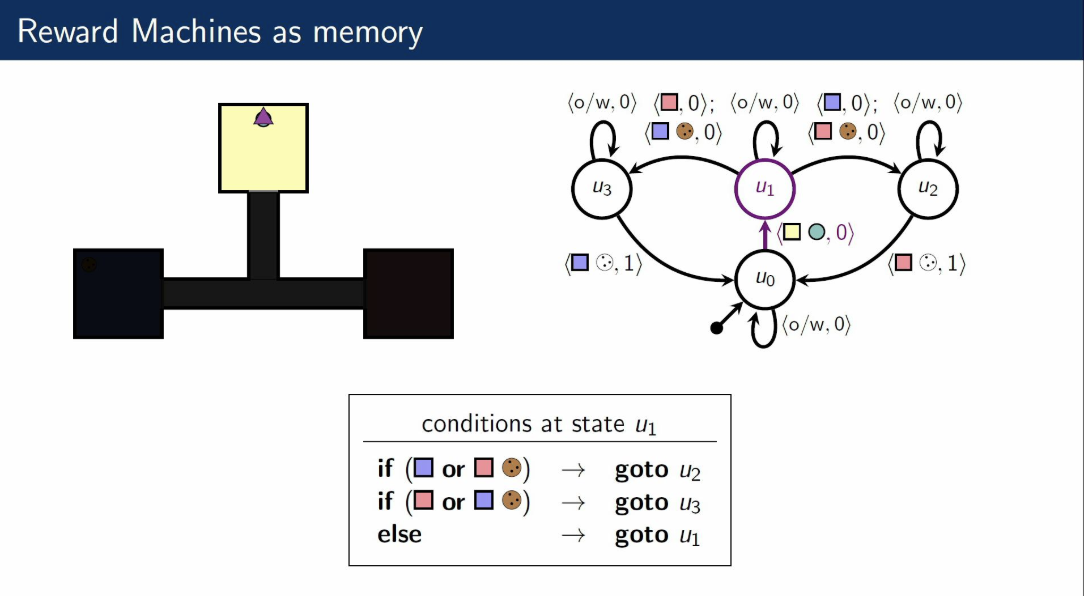
\includegraphics[width=0.7\textwidth]{figures/rm.png}
    \caption{Reward Machines as memory}
    \label{fig:rm}
\end{figure}

Introduce RM-DQN, a DQN variant that learns and uses a reward machine. \\

Overall approach:
\begin{itemize}
    \item Collect traces of experience
    \item Do optimization from this experience to propose a candidate RM
    \item Use the candidate RM to train an RL agent
    \item Add extra traces from new RL agent if the RM isn't perfect.
\end{itemize}

\spacerule